\chapter{The \FRAMEWORK}
\thispagestyle{plain}

\label{Framework}

% What does the framework do? It build meta-models that map between agent-level and system-level.
The \framework builds meta-models that map the values of agent-level control parameter values to system-level property values, and vice versa.
Learning these mappings are separate problems, which I call the \textit{forward-mapping problem} and the \textit{reverse-mapping problem}.
To solve these problems, a user of \fw ``plugs in" a regression algorithm of their choice.
The framework uses this regression algorithm to learn the mappings and then provides the user with interfaces to query them.
Once the mappings are learned, the user can query either for \textit{prediction} or for \textit{control}.
A prediction query uses the forward mapping to determine values for the expected values for system-level properties, given the system's configuration.
A control query uses the reverse mapping to suggest values for agent-level parameters, given desired values for system-level properties.
Most of the implementation details and inner workings of \fw are abstracted away from the user, who only has to attend to a limited number of configuration points.

In this chapter, I will discuss the design goals of \fw, the framework structure, software implementation details, and how well \fw conforms to the design goals.

% It frames the mapping problem into the forward mapping and the reverse mapping
% Uses a pluggable regression algorithm to solve these mapping problems

\section{Design Goals of The \framework}

% Our specific goals: provide insight and more intuitive control to agent-based models with a approach that is domain independent, algorithm independent, accurate and fast for the user.
My specific goal in designing \fw was to make the process of controlling and interacting with agent-based models more intuitive.
In addition to this central goal, \fw strives to be:
\begin{itemize}
  \item Domain-independent: The design of \fw should minimize the amount of configuration that is needed for each new domain;
  \item Algorithm-independent: Any regression algorithm should be able to be applied with \fw;
  \item Accurate: \fw should generate accurate predictions and control suggestions; and
  \item Fast for the user: Interactions with the models generated by \fw should require minimal computational time.
\end{itemize}

% Domain independence is important because the variety in which ABMs come. We want the same general approach to work for a forest fire simulation, a boid flock or particle swarm optimization.
% Algorithm independence is important because different algorithms will model different domains better. Also, as new regression techniques are implemented in the future, they can be plugged in to increase the accuracy of \fw.
Domain independence is paramount because of the variety of ABMs.
I have designed \fw in such a way that the same general approach would work for any ABM.
Also, I strove to minimize the amount of configuration that is needed to apply \fw to a new domain.
These constraints I have set on the design make \fw broadly applicable to a number of domains, without the need for in-depth domain knowledge.
To reinforce this claim, I have tested \fw on a number of diverse domains, using the same general approach for each.

Algorithm independence in a learning framework is important because different algorithms may be more effective for modeling different agent-based models.\footnote{In general, the learning algorithms that will be discussed in this dissertation will satisfy the requirements for modeling most ABMs.
However, an in-depth analysis of which types of algorithms should be used for different classes of ABMs is outside the scope of this dissertation research.}
In addition, algorithm independence allows \fw to scale with new advances in machine learning research, since future state-of-the-art regression algorithms can be used just as easily as current approaches.

Accuracy and fast user response time appear to be obvious design goals.
However, achieving these goals require sacrifices in performance in other portions of the framework.
\fw requires a significant amount of computational time to sample different configurations of the target ABM.
These large training sets can be used to build static meta-models of ABMs that are both accurate and fast to query.
In contrast, an active learning approach would be able to learn models faster, but would require more interaction with the user, increasing the user's effort.
Likewise, optimization approaches (e.g., hill climbing) could be used to generate arbitrarily accurate results, but typically require numerous iterations and would significantly increase the response time for a user's query, because each step would have to run the ABM to calculate each fitness score, which could take several seconds.
In summary, I am making the assumption that users studying ABMs with \fw are more interested in achieving more accurate results for their research and interacting with the models quickly, than spending less time sampling.


\section{Framework Structure}

% The framework is split into three phases and four major parts.
The framework is split into several phases: sampling, solving the forward-mapping problem, solving the reverse-mapping problem, querying for prediction, and querying for control (i.e., suggesting a configuration).
Figure \ref{fig:frameworkdiag} shows how the different phases interact with one another.
Sampling makes observations from the actual ABM and then feeds the newly generated data set to the forward-mapping solver.
The result of solving the forward mapping is a function $f$, which is used to predict behavior and to develop the reverse mapping $f^{-1}$.
From an external perspective, the framework only has a limited amout of input and output:
\fw takes in observations of an agent-based model and provides interfaces to query for prediction and control.
The user queries \fw to interact with the agent-based model in an intuitive way.


Many configuration points exist, which allow users of \fw to modify the behavior of the framework.
However, the individual phases take the same input and provide the same output, regardless of the configuration.
This uniformity is what makes \fw a framework and not simply a collection of algorithms.
For example, even though different regression algorithms can be used to learn the forward mapping, the forward mapping always provides predictions of how an ABM will behave, from the user's perspective.

% Each phase feeds into the next
% Many configuration points exist in which users of \fw can change the way the framework works.
% However, no matter the configuration, the input and output of each phase is the same.

% Diagram  sampling ->  [ FM / RM ] -> usage tools






\subsection{Defining System-Level Behavior Properties}
% Measurements have to be defined to tell what to sample.
The system-level properties of an ABM must be defined by the user of \fw.
The measurement of a system-level property is a statistical or mathematical calculation based on the state of the ABM over some period of time (or ``ticks'').
% Measurements must be stable (i.e., follow the laws of large numbers); they must converge over time
The one assumption made by \fw is that the measurement is \textit{stable}, meaning that as the same configuration is sampled repeatedly, the measurement's value should vary minimally.
One way to measure stability is to calculate the standard deviation of measured values of several runs of the same system.
% Wording of the measurement is important (give the example of wolves going extinct)
The need for this assumption, ways to conform to it, and a more detailed explanation of how to define system-level properties is provided in Chapter \ref{Defining}.

For example, there are several system-level behavior properties that can be measured in the Wolf Sheep Predation model.
Three of the most obvious properties are the average number of sheep, average number of wolves, and average amount of grass over a significant number of ticks.
These are measured by individually summing the number of sheep, wolves, and grass living at each time step and dividing by the number of ticks.
Although the number of sheep and wolves change rhythmically, the average values typically converge to a single value after about 10,000 ticks.


%% HACK!! I need to physically move this around
\begin{figure}[H]
\centering
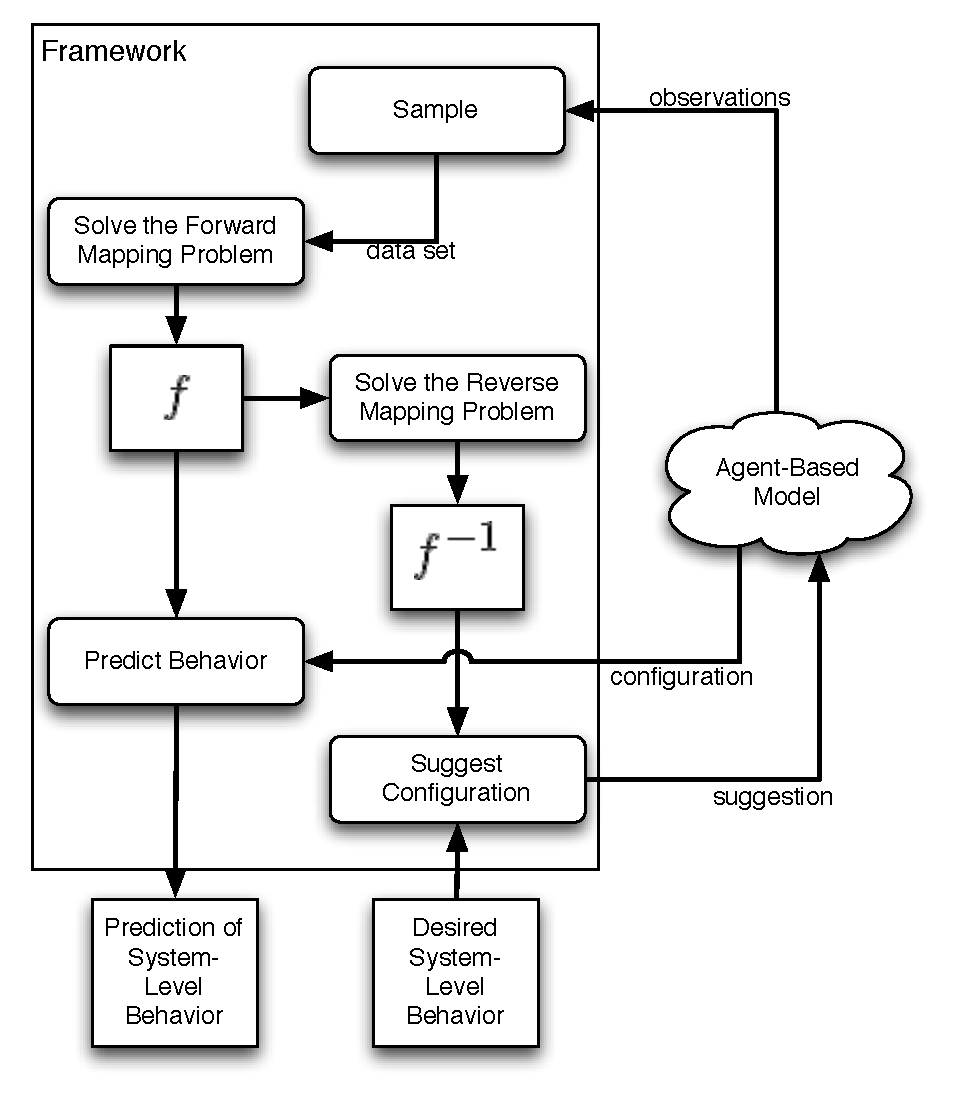
\includegraphics[scale=1]{images/framework.pdf}
\caption{An overview of the phases of \fw and how data flows among them.}
\label{fig:frameworkdiag}
\end{figure}



\subsection{Sampling}
% The first phase is sampling, in which the framework interacts with the agent-based model to generate a large enough data set for training.
The first phase is \textit{sampling}.
In this phase, numerous observations are made of different configurations of an agent-based model.
A data set is generated that contains the independent variables (the agent-level control parameter values) and the resulting system-level behaviors, for each observation.
This process can be very time-consuming, depending on several factors:
\begin{itemize}
  \item Execution time of the model -- the models will be executed numerous times, so the longer a model takes to execute, the longer the whole set of experiments will take to execute.
  \item Granularity -- more fine-grained sampling will take more time, since more points must be sampled.
  \item Dimensionality -- more agent-level control parameters result in a larger search space and naturally more points to sample.
\end{itemize}
A 120-observation sample of the NetLogo \textit{Fires} model\footnote{See Chapter \ref{Results} for detailed results.} \cite{fires} requires roughly thirty seconds\footnote{Most experiments are executed on a 3.0 Ghz Pentium 4 running Arch Linux.} to generate.
A large sample of 50,000 observations of a Reynolds boid flock \cite{reynolds1987} took approximately four days.

The user is required to have enough understanding of the domain to specify to \fw which  ranges of values should be sampled.
\fw is not able to automatically infer which value ranges are interesting, so these must be explicitly defined.

This sampling process is easily parallelizable.
Since each experiment is independent of the others, the set of all experiments can be segmented among a number of systems and processors to significantly reduce the computation time.
Once all of the experiments are completed, the results can be merged into one data set.

% For this dissertation, we either use a random sampling method or a systematic sampling method
% Future work: plug in different advanced sampling methods
For the purposes of this dissertation, I limit \fw to use a simple random sampling method (i.e., randomly select points within a specified range) or a systematic sampling method (i.e., given ranges, sample evenly spaced points).
I acknowledge that intelligent sampling strategies could improve the performance of the framework, and such strategies could be the focus of future work.


\subsection{The Forward-Mapping Problem}

% The second phase is learning the forward and reverse mapping.
% This is the main focus of the learning framework.

% Explain the forward mapping problem; give an example [figure]

The \textit{forward-mapping problem} is to develop a function $f: \mathbb{R}^n \rightarrow \mathbb{R}$ that maps a provided configuration vector $\mathbf x = \{x_1, x_2, ..., x_n \}$ to several system-level behavior properties $\hat {\mathbf y}$:
\[f(\mathbf x) \rightarrow  \hat{\mathbf y}\]
The set of values $\mathbf x$ consists of all of the agent-level parameters (independent variables) in the data set provided by the sampling phase.
An individual mapping is learned for each system-level behavior measurement provided by the user.
% The forward mapping is a straightforward regression problem ... Assuming this is a many-to-one relationship (due to the correct definition of the measurement)

This problem is solved with straightforward regression, such as k-nearest neighbor.
% A regression algorithm needs to be initialized with the data set (if necessary). For example, a linear regression approach would solve the least-squares problem to generate the model. Meanwhile, something like KNN has no initialization time.
In this phase of \fw, the regression algorithm is first ``initialized," if necessary.
For example, linear regression would need to solve the least-squares problem.
On the other hand, an algorithm like k-nearest neighbor would not necessarily need to initialize anything because it scans the data set per query.
% The forward mapping problem returns an object that can be queried for configuration vector x, and returns system-level property y.
Then, the forward mapping can be used to predict values for configurations that have not been sampled.

Once this phase is completed, the user is presented with $f$, an interface to the mapping built by the regression algorithm.
The forward mapping is primarily used to \textit{predict} what the system-level property values will be, given the system's configuration.
For example, a learned mapping could be used to determine the average number of sheep given a configuration vector, without having to run the system.
Some sample predictions, given particular system configurations, are shown in Table \ref{table:ws_predictions}.
The values for a system configuration represent \textit{grass-regrowth-time}, \textit{sheep-gain-from-food}, \textit{wolf-gain-from-food}, \textit{sheep-reproduce}, and \textit{wolf-reproduce}, respectively.

\begin{table}[ht]
  \caption{Sample Predictions of Behavior in the Wolf Sheep Predation Model}
  \centering
  \begin{tabular}{c c c c}
    \hline \hline
    Configuration & Average \# Sheep & Average \# Wolves & Average \# Grass \\
    \hline
    $(30, 4, 20, 4, 5)$ & 162.8 & 76.1 & 964.8 \\
    $(30, 3, 26, 7, 5)$ & 122.8 & 90.4 & 1135.2 \\
    $(14, 3, 26, 7, 5)$ & 144.3 & 163.8 & 1621.4 \\
    $(5, 3, 17, 7, 5)$ & 946.9 & 3.4 & 1065.4 \\
    \hline
  \end{tabular}
  \label{table:ws_predictions}
\end{table}


A more in-depth definition of the forward-mapping problem, specific examples of regression methods used in \fw, and the role of regression are given in Chapter \ref{ForwardMapping}.


\subsection{The Reverse-Mapping Problem}

% Explain the reverse mapping problem; give an example [figure]


The \textit{reverse-mapping problem} is to produce a mapping $ f^{-1}: \mathbb{R} \rightarrow \hat S$ from given system-level behavior properties $\mathbf y$ to a set of
configurations $ \hat S = \{ \mathbf {\hat x} | f( \mathbf {\hat x}) = \mathbf y \}$
(i.e., $S$ is the set of behaviors that will produce behavior $\mathbf y$):
\[f^{-1}(\mathbf y) \rightarrow \hat S\]

% The reverse mapping is an "inverted" regression problem.

% We invert the forward mapping
% Inverted regression means f^-1 (building an inverted mapping)
The problem of developing the mapping $f^{-1}$ is what I call an ``inverted regression problem" and has many unique challenges.
The main challenge is that $f^{-1}$ does not, in general, describe a functional mapping:
$f^{-1}$ describes a one-to-many relationship, since $f$ is many-to-one.
Therefore, \fw cannot use standard regression techniques to solve this problem.
Instead, the default behavior of \fw is to approximate the inverse of the forward mapping, using a novel method that I developed called \textit{simplicial complex inversion}.
This approach has the benefit of using the forward mapping to develop the reverse mapping, so no additional inputs from the user or additional data samples are needed.
% Elude that we will discuss our particular solutions to these problems in later chapters

The reverse mapping can be used to suggest a system configuration that will exhibit a specific set of system-level properties.
I call this process \textit{control} of the ABM, since it is controlling the ABM at the system level by suggesting configurations.
For example, the reverse mapping could be used to suggest a configuration of $(30, 4, 20, 4, 5)$  for a desired system-level property of 162.8 average sheep (see Table \ref{table:ws_predictions}).
However, using the reverse mapping is more involved than using the forward mapping, because $f^{-1}$ returns a set of possible solutions, not a single suggestion.
If the mapping is to be used for control, any configuration in this set will satisfy the system-level requirements.
Therefore, an additional step must be taken to extract a point from the set if it is to be used to control an ABM.

The implementation details of developing reverse mappings and how to use the reverse mappings are discussed in Chapter \ref{ReverseMapping}.


% Explain how the maps are queried.
% Querying the forward mapping (example)
% Querying the reverse mapping (example)

% Possible uses: prediction and control



\subsection{Summary of Configuration Points}

% Sampling methodology
% Measurements
% Forward Mapping Algorithm
% Reverse Mapping Algorithm
The following is a summary of the configuration points discussed in this section.
For each new domain, the user must specify the following:
\begin{itemize}
   \item A list of agent-level control parameters, and the ranges within which they should be sampled.
   \item A list of system-level behavior properties and a process for measuring them.
\end{itemize}

In addition, the user may configure the following if they wish to modify the default behavior of \fw:
\begin{itemize}
   \item The sampling strategy (default: random sampling).
   \item The regression algorithm to be used for the forward mapping (defaults: k-nearest neighbor, locally weighted linear regression, or nonlinear regression).
   \item The method for the reverse mapping (default: approximate the inverse of the forward mapping).
\end{itemize}


\section{Software Implementation Details}
So far, I have discussed \fw abstractly, avoiding specific implementation details, because the framework is a methodology and could be reimplemented in a number of different ways or to work with a number of different ABM simulation systems.
In this section, I discuss the details of my proof-of-concept implementation that was used to run many of the experiments documented in Chapter \ref{Results}.

% Most of the software is implemented in python, but the interaction with NetLogo is handled with Java, so that I can access the Java API.
I have tested \fw with NetLogo\footnote{NetLogo is discussed in more detail in Chapter \ref{Background}.} domains; however, any agent-based modeling system could be used.
The rest of the framework is implemented in Python.
Each step of \fw returns its result as a file, so that it can be passed to the next step or saved for later use.
For example, the forward mapping writes the model to a file so that it can be used by both the prediction script and the reverse mapping script.

Since each domain has different variable names and nuances, the user must implement a Java program that interacts with NetLogo's API.
An abstract base class for interaction is provided to guide the development of this program.
Next, the user lists the configuration parameters and the ranges of these values so that the sampling can begin.
Measuring the system-level parameters can either be calculated within NetLogo or in Java.
For example, I modified the standard Wolf Sheep Predation model to keep track of the number of sheep at each tick.
Then, to extract the value, NetLogo's API is used to retrieve the sum of the sheep divided by the number of ticks.
A similar calculation could be performed within a Java program by retrieving each of these values individually, then performing statistics on them.
Performing the statistics calculations in Java has the benefit of not having to change the NetLogo ABM source code.


During sampling, the data set is written to a file, row by row.
Therefore, the results of several instances of the sampling, executing on different machines, can be easily concatenated.
%An example of a sampling program for Wolf Sheep predation is given in Appendix \ref{SamplingProgram}.


The regression algorithms used with \fw must conform to a standard API
%\footnote{The specification for the standard regression algorithm interface is given in Appendix \ref{RegressionInterface}.}
and are passed as arguments into the forward mapping, reverse mapping and prediction scripts.
Therefore, no configuration of these core scripts is needed, since they are ``pluggable."

An overarching ``master script," written in Python, runs all steps automatically, limiting the amount of direct interaction with the framework software.

In addition to the core framework software, I have developed a toolkit that queries the models generated by the forward- and reverse-mapping models.
The core tools include:
\begin{itemize}
   \item Query the forward mapping for a prediction by passing in a configuration,
   \item Query the reverse mapping for a set of possible solutions by passing in a desired system-level behavior configuration,
   \item Visualize the mappings.
\end{itemize}

% Give a list of agent-level variable ranges/steps
% Generate the experiments list
% Samples a NetLogo ABM with Java API, given the list of experiments, save the results
% Interact with the forward mapping regression algorithm with a python module interface
% Interact with the reverse mapping approach (discussed more in Chapter X) with a python module interface
% Different tools for selecting solutions and visualizing slices are separate python scripts.

% An overarching "master script" written in python that glues these together and automatically transitions from one to another. Each stage can be performed one by one

% More about NetLogo is covered in Background.





\section{Analysis of \fw  vs. the Design Goals}
In this section, I align the actual implementation of \fw with the design goals.

% for my reference...
%  \item Domain independent -- the design of \fw should minimize the amount of configuration for each domain,
%  \item Algorithm independent -- any regression algorithm should be able to be plugged into \fw,
%  \item Accurate -- \fw should generate accurate predictions and control suggestions,
%  \item Fast for the user -- interactions with the models generated by \fw should require minimal computational time.


% Our framework is domain independent, because it reduces the forward mapping problem to a classical regression problem of learning the correlation between the agent-level parameters and the system-level properties..
% We introduce a domain-independent approach to solve the reverse mapping problem that uses standard regression to build a space of configurations that would produce desired behavior.
\textit{Domain independence}---
My framework's implementation is domain-independent, to an extent. \fw reduces the forward-mapping problem to a classical regression problem of learning the correlation between the agent-level parameters and the system-level properties.
My reverse-mapping problem solution is also domain-independent because it interacts exclusively with the forward mapping, which is domain-independent.
However, my implementation of \fw still requires the user to specify the agent-level parameters and how to measure the system-level properties.
This is a reasonable requirement, since automatically detecting configuration points and having a computer determine the behaviors of interest in an ABM would be a challenging unsupervised learning problem.

% Our framework is algorithm independent, because any regression algorithm (e.g., ...) can be used to develop the forward mapping and the reverse mapping
\textit{Algorithm independence}---
Any regression algorithm can be plugged into my implementation, as long as it conforms to the standard API.
A simple Python wrapper can be written to adapt an existing third-party regression algorithm to work with my implementation of \fw.
My  default process of inverted regression requires nothing special of the regression algorithm, because the inversion learning process uses the algorithm's standard forward-mapping behavior.

% Our framework is as accurate as the regression algorithms used and the data set sampled from the agent-based model. /elaborate/
% In general, I prefer spending longer sampling to generate an exhaustive data set increase accuracy and reducing user interaction delays when querying for a prediction or a suggestion for controlling.
% This shifts most of the computation time offline, instead of online, reducing user interaction time when querying the forward or reverse mappings.
\textit{Accuracy}---
No extra error is incurred by \fw itself;
the accuracy of \fw depends on the regression algorithm used and the amount of time spent sampling.
If \fw is not providing accurate results with state-of-the-art regression algorithms, either the correlations cannot be learned with current technology or not enough time has been spent sampling.


\textit{Fast for the user}---
Most computation time is spent sampling and learning the models.
These operations are offline and do not affect the response time of real-time interaction with the user.
The response time of the forward mapping and the reverse mapping are depend on the running time of the regression algorithms, but typically require less than a few seconds.





